\subsection{Theory}

Registration is the process of finding a spatial transformation that aligns two point sets or 3D point clouds. The goal is to find the relative position and orientation of the different acquired views in a global coordinate framework. The intersection between the different point cloud data views must overlap perfectly. This problem is often referred as pairwise registration.
The goal is to find a rigid body 4x4 transformation matrix (\ref{equation:rigid_transformation_matrix}) which is composed of a 3x3 rotation matrix \textbf{R} and a 3x1 translation vector \textbf{t}. \textit{Rigid body} means that the proportion of the 'body', e.g. the point cloud, are preserved. This transformation is applied to one of the point cloud (the source) in order to be perfectly aligned with the other point cloud (the target). Figure \ref{figure:transformation_matrix} illustrates the problem.

\begin{figure}[H]
    \centering
    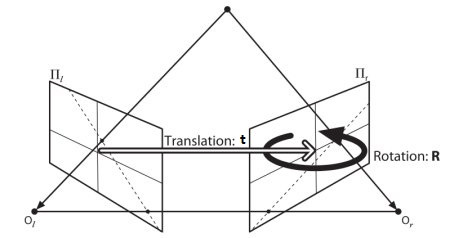
\includegraphics[width=0.65\textwidth]{images/registration/essential_matrix.jpg}
    \caption{Illustration of the registration problem. \textbf{R} and \textbf{t} have to be found to align two different views of the same scene. $O_l$ and $O_r$ are the camera centres. Source: \cite{noauthor_epipolar_nodate}}
    \label{figure:transformation_matrix}
\end{figure}

\begin{equation}
\label{equation:rigid_transformation_matrix}
\mathbf{M}=\left[\begin{array}{ll}
{\mathbf{R}} & {\mathbf{t}} \\
{\mathbf{0}^T} & {1}
\end{array}\right]
\end{equation}


The following matrices defines the rotation around the x,y and z-axis, explained in \cite{noauthor_rotation_2020}.

\begin{equation}
\mathbf{R}_{x}=\left[\begin{array}{ccc}
{1} & {0} & {0} \\
{0} & {\cos \theta_{x}} & {-\sin \theta_{x}} \\
{0} & {\sin \theta_{x}} & {\cos \theta_{x}}
\end{array}\right], \mathbf{R}_{y}=\left[\begin{array}{ccc}
{\cos \theta_{y}} & {0} & {\sin \theta_{y}} \\
{0} & {1} & {0} \\
{-\sin \theta_{y}} & {0} & {\cos \theta_{y}}
\end{array}\right], \mathbf{R}_{z}=\left[\begin{array}{ccc}
{\cos \theta_{z}} & {-\sin \theta_{z}} & {0} \\
{\sin \theta_{z}} & {\cos \theta_{z}} & {0} \\
{0} & {0} & {1}
\end{array}\right]
\end{equation}

\newpage
where:
\begin{itemize}
    \item $\theta_{x}$ is the rotation around the x-axis
    \item $\theta_{y}$ is the rotation around the y-axis
    \item $\theta_{z}$ is the rotation around the z-axis
\end{itemize}

The general rotation matrix can be obtained by multiplying these three rotation matrices.
% \begin{gather}
% \mathbf{R}=\mathbf{R}_{z} \mathbf{R}_{y}\mathbf{R}_{x}\\
% =\left[\begin{array}{ccc}
% {\cos \theta_{y} \cos \theta_{z}} & {-\cos \theta_{y} \sin \theta_{z}} & {\sin \theta_{y}} \\
% {\cos \theta_{x} \sin \theta_{z}+\cos \theta_{z} \sin \theta_{x} \sin \theta_{y}} & {\cos \theta_{x} \cos \theta_{z}-\sin \theta_{x} \sin \theta_{y} \sin \theta_{z}} & {-\cos \theta_{y} \sin \theta_{x}} \\
% {\sin \theta_{x} \sin \theta_{z}} & {-\cos \theta_{x} \cos \theta_{z} \sin \theta_{y}} & {\cos \theta_{z} \sin \theta_{x}+\cos \theta_{x} \sin \theta_{y} \sin \theta_{z}} & {\cos \theta_{x} \cos \theta_{y}}
% \end{array}\right]
% \end{gather}

\begin{gather}
\mathbf{R}=\mathbf{R}_{z} \mathbf{R}_{y}\mathbf{R}_{x}\\
=\left[\begin{array}{ccc}\cos \theta_{z} \cos \theta_{y} & \cos \theta_{z} \sin \theta_{y} \sin \theta_{x}-\sin \theta_{z} \cos \theta_{x} & \cos \theta_{z} \sin \theta_{y} \cos \theta_{x}+\sin \theta_{z} \sin \theta_{x} \\ \sin \theta_{z} \cos \theta_{y} & \sin \theta_{z} \sin \theta_{y} \sin \theta_{x}+\cos \theta_{z} \cos \theta_{x} & \sin \theta_{z} \sin \theta_{y} \cos \theta_{x}-\cos \theta_{z} \sin \theta_{x} \\ -\sin \theta_{y} & \cos \theta_{y} \sin \theta_{x} & \cos \theta_{y} \cos \theta_{x}\end{array}\right]
\end{gather}

The translation vector is defined as follow:

\begin{equation}
\mathbf{t}=\left[\begin{array}{ll}
t_x \\
t_y \\
t_z
\end{array}\right]
\end{equation}

where:
\begin{itemize}
    \item $t_x$ is the translation along the x-axis
    \item $t_y$ is the translation along the y-axis
    \item $t_z$ is the translation along the z-axis
\end{itemize}